
\documentclass[14pt]{extbook}
%General Packages
\usepackage{multicol, enumerate, enumitem, hyperref, color, soul, setspace, parskip, fancyhdr}

%Math Packages
\usepackage{amssymb, amsthm, amsmath, bbm, latexsym, units, mathtools}

%All math in Display Style
\everymath{\displaystyle}

% Packages with additional options
%\usepackage[T1]{fontenc}
\usepackage[headsep=0.5cm,headheight=12pt, left=1 in,right= 1 in,top= 1 in,bottom= 1 in]{geometry}
\usepackage[usenames,dvipsnames]{xcolor}

% SageTeX
\usepackage{sagetex}

% Package to use the command below to create lines between items
\usepackage{dashrule}
\newcommand{\litem}[1]{\item#1\hspace*{-1cm}\rule{\textwidth}{0.4pt}}

\pagestyle{fancy}
\lhead{}
\chead{Final Exam}
\rhead{}
\lfoot{Spring 2020}
\cfoot{}
\rfoot{Version A}

\begin{document}
\pagestyle{fancy}

\begin{sagesilent}
load("../Code/pythonImports.sage")
load("../Code/intervalMaskingMethod.sage")
load("../Code/keyGeneration.sage")
load("../Code/commonlyUsedFunctions.sage")
keyFileName = "FinalExam"
version = "A"
\end{sagesilent}

\begin{enumerate}


  \begin{sagesilent}
  moduleNumber="6"
  problemNumber=1
  load("../Code/06polynomial/polyGraphToFunction.sage")
  \end{sagesilent}

  \litem{ \sage{displayStem}

   \begin{center}
       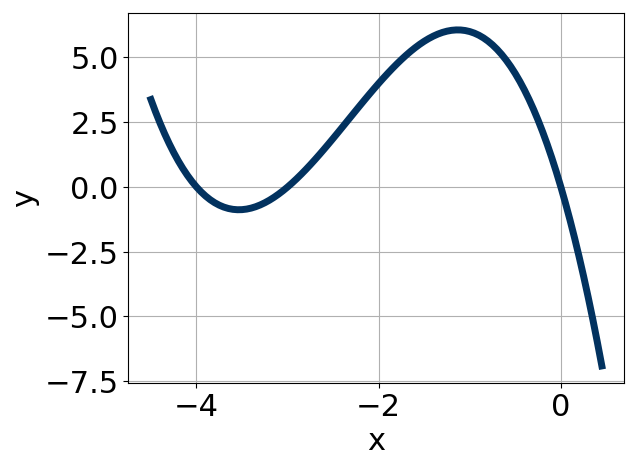
\includegraphics[width=0.5\textwidth]{../Figures/polyGraphToFunctionA.png}
   \end{center}

  	\begin{enumerate}[label=\Alph*.]
    \item \( \sage{choices[0]} \)
    \item \( \sage{choices[1]} \)
    \item \( \sage{choices[2]} \)
    \item \( \sage{choices[3]} \)
    \item \( \sage{choices[4]} \)
  	\end{enumerate}
  }

  \begin{sagesilent}
  moduleNumber="7"
  problemNumber=2
  load("../Code/07rational/rationalGraphToEquation.sage")
  \end{sagesilent}

  \litem{ \sage{displayStem}

   \begin{center}
       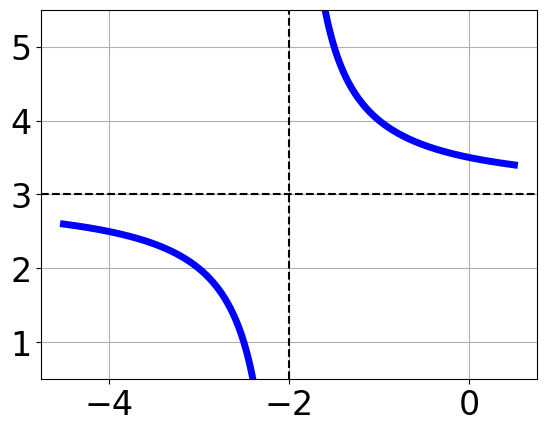
\includegraphics[width=0.5\textwidth]{../Figures/rationalGraphToEquationA.png}
   \end{center}

  	\begin{enumerate}[label=\Alph*.]
    \item \( \sage{choices[0]} \)
    \item \( \sage{choices[1]} \)
    \item \( \sage{choices[2]} \)
    \item \( \sage{choices[3]} \)
    \item \( \sage{choices[4]} \)
  	\end{enumerate}
  }

\begin{sagesilent}
moduleNumber="6"
problemNumber=3
load("../Code/06polynomial/polyZeroBehavior.sage")
\end{sagesilent}

\litem{ \sage{displayStem}

\[ \sage{displayProblem} \]

\begin{enumerate}[label=\Alph*.]
    \begin{multicols}{2}
	      \item 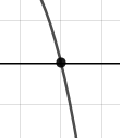
\includegraphics[width = 0.3\textwidth]{../Figures/polyZeroBehaviorAA.png}
		    \item 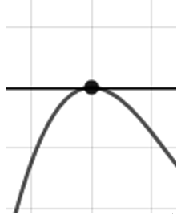
\includegraphics[width = 0.3\textwidth]{../Figures/polyZeroBehaviorBA.png}
		    \item 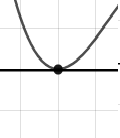
\includegraphics[width = 0.3\textwidth]{../Figures/polyZeroBehaviorCA.png}
		    \item 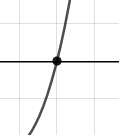
\includegraphics[width = 0.3\textwidth]{../Figures/polyZeroBehaviorDA.png}
    \end{multicols}
        \item \text{None of the above.}
\end{enumerate}
}
\begin{sagesilent}
moduleNumber="6"
problemNumber=4
load("../Code/06polynomial/constructPolyRationals.sage")
\end{sagesilent}

\litem{ \sage{displayStem}

   \[ \sage{displayProblem} \]

  	\begin{enumerate}[label=\Alph*.]
    \item \( \sage{choices[0]} \)
    \item \( \sage{choices[1]} \)
    \item \( \sage{choices[2]} \)
    \item \( \sage{choices[3]} \)
    \item \( \sage{choices[4]} \)
  	\end{enumerate}
  }

  \begin{sagesilent}
  moduleNumber="4"
  problemNumber=5
  load("../Code/04quadratic/quadraticGraphToEquation.sage")
  \end{sagesilent}

  \litem{ \sage{displayStem}

   \begin{center}
       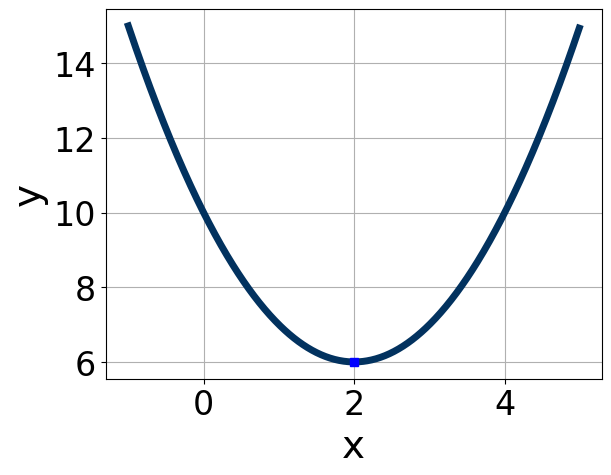
\includegraphics[width=0.5\textwidth]{../Figures/quadraticGraphToEquationA.png}
   \end{center}

  	\begin{enumerate}[label=\Alph*.]
    \item \( \sage{choices[0]} \)
    \item \( \sage{choices[1]} \)
    \item \( \sage{choices[2]} \)
    \item \( \sage{choices[3]} \)
    \item \( \sage{choices[4]} \)
  	\end{enumerate}
  }
\begin{sagesilent}
moduleNumber="5"
problemNumber=6
load("../Code/05radical/solveRadicalLinear.sage")
\end{sagesilent}

\litem{ \sage{displayStem}

   \[ \sage{displayProblem} \]

  	\begin{enumerate}[label=\Alph*.]
    \item \( \sage{choices[0]} \)
    \item \( \sage{choices[1]} \)
    \item \( \sage{choices[2]} \)
    \item \( \sage{choices[3]} \)
    \item \( \sage{choices[4]} \)
  	\end{enumerate}
  }
\begin{sagesilent}
moduleNumber="1"
problemNumber=7
load("../Code/01realComplex/subgroupReal.sage")
\end{sagesilent}

\litem{ \sage{displayStem}

   \[ \sage{displayProblem} \]

  	\begin{enumerate}[label=\Alph*.]
    \item \( \sage{choices[0]} \)
    \item \( \sage{choices[1]} \)
    \item \( \sage{choices[2]} \)
    \item \( \sage{choices[3]} \)
    \item \( \sage{choices[4]} \)
  	\end{enumerate}
  }
\begin{sagesilent}
moduleNumber="3"
problemNumber=8
load("../Code/03inequality/solveCompoundAND.sage")
\end{sagesilent}

\litem{ \sage{displayStem}

   \[ \sage{displayProblem} \]

  	\begin{enumerate}[label=\Alph*.]
    \item \( \sage{choices[0]} \)
    \item \( \sage{choices[1]} \)
    \item \( \sage{choices[2]} \)
    \item \( \sage{choices[3]} \)
    \item \( \sage{choices[4]} \)
  	\end{enumerate}
  }
\begin{sagesilent}
moduleNumber="2"
problemNumber=9
load("../Code/02linear/solveRationalLinear.sage")
\end{sagesilent}

\litem{ \sage{displayStem}

   \[ \sage{displayProblem} \]

  	\begin{enumerate}[label=\Alph*.]
    \item \( \sage{choices[0]} \)
    \item \( \sage{choices[1]} \)
    \item \( \sage{choices[2]} \)
    \item \( \sage{choices[3]} \)
    \item \( \sage{choices[4]} \)
  	\end{enumerate}
  }
\begin{sagesilent}
moduleNumber="2"
problemNumber=10
load("../Code/02linear/solveRationalLinear.sage")
\end{sagesilent}

\litem{ \sage{displayStem}

   \[ \sage{displayProblem} \]

  	\begin{enumerate}[label=\Alph*.]
    \item \( \sage{choices[0]} \)
    \item \( \sage{choices[1]} \)
    \item \( \sage{choices[2]} \)
    \item \( \sage{choices[3]} \)
    \item \( \sage{choices[4]} \)
  	\end{enumerate}
  }

\begin{sagesilent}
moduleNumber="5"
problemNumber=11
load("../Code/05radical/radicalEquationToGraph.sage")
\end{sagesilent}

\litem{ \sage{displayStem}

\[ \sage{displayProblem} \]

\begin{enumerate}[label=\Alph*.]
    \begin{multicols}{2}
	      \item 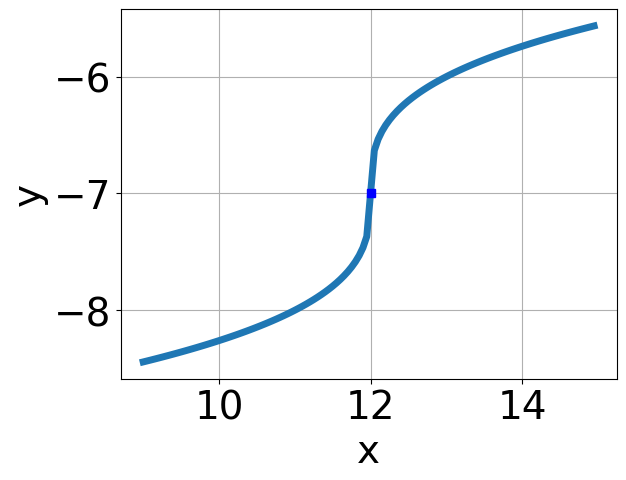
\includegraphics[width = 0.3\textwidth]{../Figures/radicalEquationToGraphAA.png}
		    \item 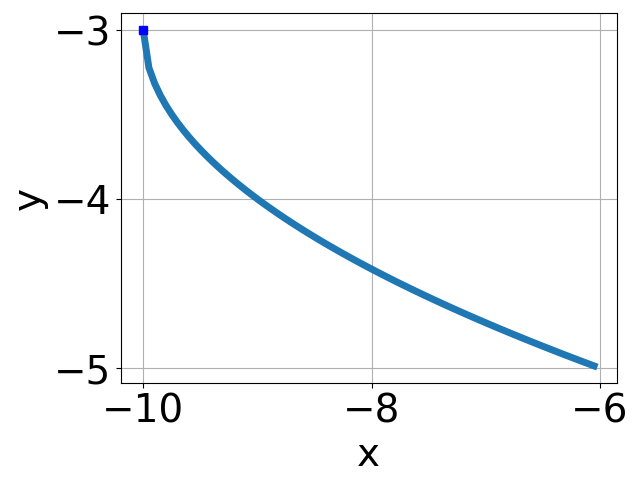
\includegraphics[width = 0.3\textwidth]{../Figures/radicalEquationToGraphBA.png}
		    \item 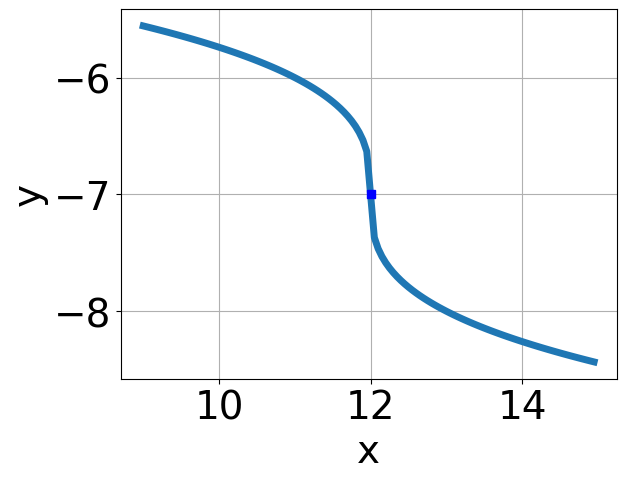
\includegraphics[width = 0.3\textwidth]{../Figures/radicalEquationToGraphCA.png}
		    \item 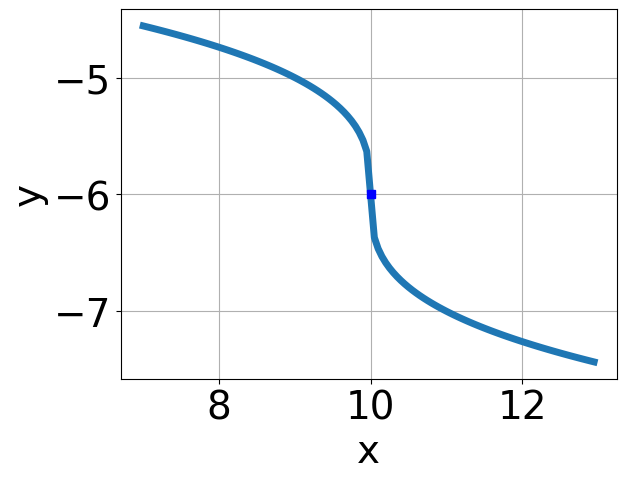
\includegraphics[width = 0.3\textwidth]{../Figures/radicalEquationToGraphDA.png}
    \end{multicols}
        \item \text{None of the above.}
\end{enumerate}
}
\begin{sagesilent}
moduleNumber="2"
problemNumber=12
load("../Code/02linear/linearParOrPer.sage")
\end{sagesilent}

\litem{ \sage{displayStem}

   \[ \sage{displayProblem} \]

  	\begin{enumerate}[label=\Alph*.]
    \item \( \sage{choices[0]} \)
    \item \( \sage{choices[1]} \)
    \item \( \sage{choices[2]} \)
    \item \( \sage{choices[3]} \)
    \item \( \sage{choices[4]} \)
  	\end{enumerate}
  }
\begin{sagesilent}
moduleNumber="2"
problemNumber=13
load("../Code/02linear/linearTwoPoints.sage")
\end{sagesilent}

\litem{ \sage{displayStem}

   \[ \sage{displayProblem} \]

  	\begin{enumerate}[label=\Alph*.]
    \item \( \sage{choices[0]} \)
    \item \( \sage{choices[1]} \)
    \item \( \sage{choices[2]} \)
    \item \( \sage{choices[3]} \)
    \item \( \sage{choices[4]} \)
  	\end{enumerate}
  }
\begin{sagesilent}
moduleNumber="1"
problemNumber=14
load("../Code/01realComplex/orderOfOperations.sage")
\end{sagesilent}

\litem{ \sage{displayStem}

   \[ \sage{displayProblem} \]

  	\begin{enumerate}[label=\Alph*.]
    \item \( \sage{choices[0]} \)
    \item \( \sage{choices[1]} \)
    \item \( \sage{choices[2]} \)
    \item \( \sage{choices[3]} \)
    \item \( \sage{choices[4]} \)
  	\end{enumerate}
  }

\begin{sagesilent}
moduleNumber="4"
problemNumber=15
load("../Code/04quadratic/quadraticEquationToGraph.sage")
\end{sagesilent}

\litem{ \sage{displayStem}

\[ \sage{displayProblem} \]

\begin{enumerate}[label=\Alph*.]
    \begin{multicols}{2}
	      \item 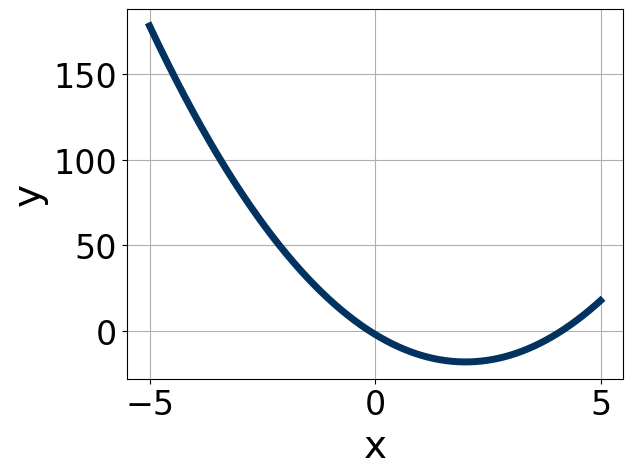
\includegraphics[width = 0.3\textwidth]{../Figures/quadraticEquationToGraphAA.png}
		    \item 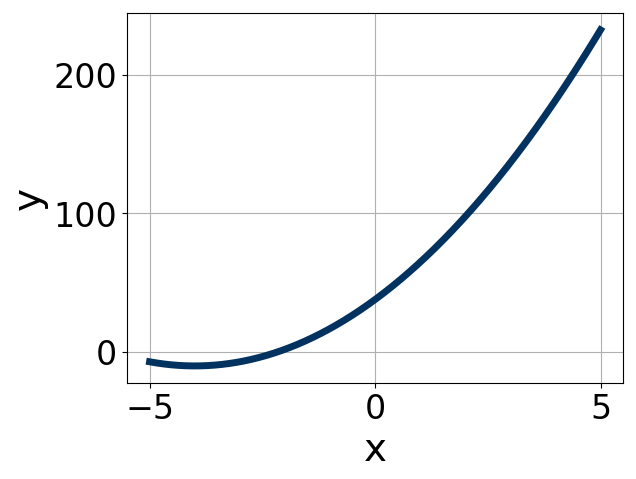
\includegraphics[width = 0.3\textwidth]{../Figures/quadraticEquationToGraphBA.png}
		    \item 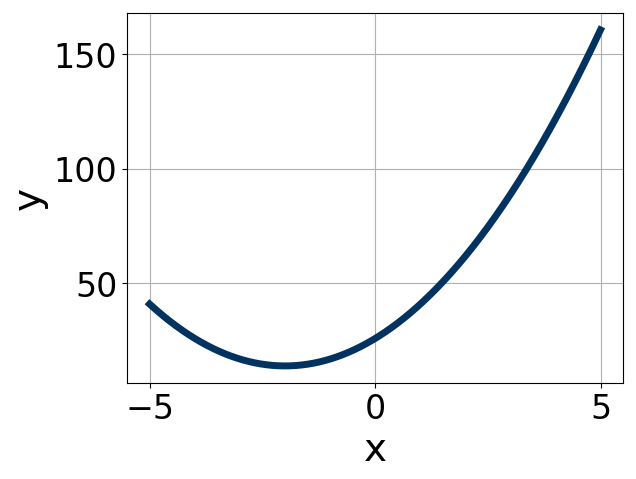
\includegraphics[width = 0.3\textwidth]{../Figures/quadraticEquationToGraphCA.png}
		    \item 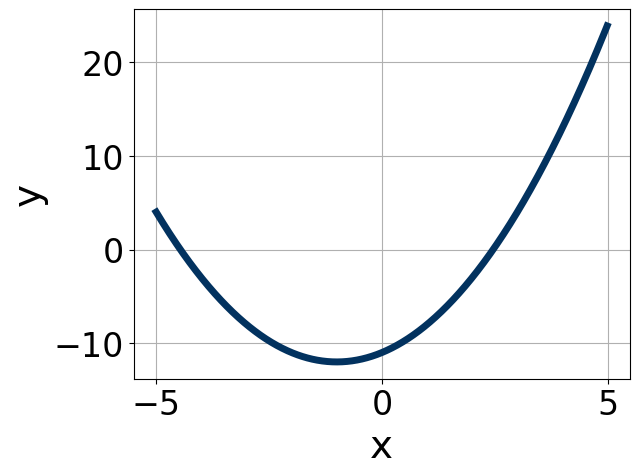
\includegraphics[width = 0.3\textwidth]{../Figures/quadraticEquationToGraphDA.png}
    \end{multicols}
        \item \text{None of the above.}
\end{enumerate}
}
\begin{sagesilent}
moduleNumber="5"
problemNumber=16
load("../Code/05radical/domainRadical.sage")
\end{sagesilent}

\litem{ \sage{displayStem}

   \[ \sage{displayProblem} \]

  	\begin{enumerate}[label=\Alph*.]
    \item \( \sage{choices[0]} \)
    \item \( \sage{choices[1]} \)
    \item \( \sage{choices[2]} \)
    \item \( \sage{choices[3]} \)
    \item \( \sage{choices[4]} \)
  	\end{enumerate}
  }
\begin{sagesilent}
moduleNumber="3"
problemNumber=17
load("../Code/03inequality/solveRationalInequality.sage")
\end{sagesilent}

\litem{ \sage{displayStem}

   \[ \sage{displayProblem} \]

  	\begin{enumerate}[label=\Alph*.]
    \item \( \sage{choices[0]} \)
    \item \( \sage{choices[1]} \)
    \item \( \sage{choices[2]} \)
    \item \( \sage{choices[3]} \)
    \item \( \sage{choices[4]} \)
  	\end{enumerate}
  }
\begin{sagesilent}
moduleNumber="4"
problemNumber=18
load("../Code/04quadratic/quadraticFormula.sage")
\end{sagesilent}

\litem{ \sage{displayStem}

   \[ \sage{displayProblem} \]

  	\begin{enumerate}[label=\Alph*.]
    \item \( \sage{choices[0]} \)
    \item \( \sage{choices[1]} \)
    \item \( \sage{choices[2]} \)
    \item \( \sage{choices[3]} \)
    \item \( \sage{choices[4]} \)
  	\end{enumerate}
  }
\begin{sagesilent}
moduleNumber="1"
problemNumber=19
load("../Code/01realComplex/divideComplex.sage")
\end{sagesilent}

\litem{ \sage{displayStem}

   \[ \sage{displayProblem} \]

  	\begin{enumerate}[label=\Alph*.]
    \item \( \sage{choices[0]} \)
    \item \( \sage{choices[1]} \)
    \item \( \sage{choices[2]} \)
    \item \( \sage{choices[3]} \)
    \item \( \sage{choices[4]} \)
  	\end{enumerate}
  }
\begin{sagesilent}
moduleNumber="8"
problemNumber=20
load("../Code/08logExp/domainRangeExp.sage")
\end{sagesilent}

\litem{ \sage{displayStem}

   \[ \sage{displayProblem} \]

  	\begin{enumerate}[label=\Alph*.]
    \item \( \sage{choices[0]} \)
    \item \( \sage{choices[1]} \)
    \item \( \sage{choices[2]} \)
    \item \( \sage{choices[3]} \)
    \item \( \sage{choices[4]} \)
  	\end{enumerate}
  }
\begin{sagesilent}
moduleNumber="7"
problemNumber=21
load("../Code/07rational/solveRationalQuadratic.sage")
\end{sagesilent}

\litem{ \sage{displayStem}

   \[ \sage{displayProblem} \]

  	\begin{enumerate}[label=\Alph*.]
    \item \( \sage{choices[0]} \)
    \item \( \sage{choices[1]} \)
    \item \( \sage{choices[2]} \)
    \item \( \sage{choices[3]} \)
    \item \( \sage{choices[4]} \)
  	\end{enumerate}
  }
\begin{sagesilent}
moduleNumber="3"
problemNumber=22
load("../Code/03inequality/solveIntegerInequality.sage")
\end{sagesilent}

\litem{ \sage{displayStem}

   \[ \sage{displayProblem} \]

  	\begin{enumerate}[label=\Alph*.]
    \item \( \sage{choices[0]} \)
    \item \( \sage{choices[1]} \)
    \item \( \sage{choices[2]} \)
    \item \( \sage{choices[3]} \)
    \item \( \sage{choices[4]} \)
  	\end{enumerate}
  }
\begin{sagesilent}
moduleNumber="8"
problemNumber=23
load("../Code/08logExp/domainRangeLog.sage")
\end{sagesilent}

\litem{ \sage{displayStem}

   \[ \sage{displayProblem} \]

  	\begin{enumerate}[label=\Alph*.]
    \item \( \sage{choices[0]} \)
    \item \( \sage{choices[1]} \)
    \item \( \sage{choices[2]} \)
    \item \( \sage{choices[3]} \)
    \item \( \sage{choices[4]} \)
  	\end{enumerate}
  }
\begin{sagesilent}
moduleNumber="8"
problemNumber=24
load("../Code/08logExp/solveExpDifferentBases.sage")
\end{sagesilent}

\litem{ \sage{displayStem}

   \[ \sage{displayProblem} \]

  	\begin{enumerate}[label=\Alph*.]
    \item \( \sage{choices[0]} \)
    \item \( \sage{choices[1]} \)
    \item \( \sage{choices[2]} \)
    \item \( \sage{choices[3]} \)
    \item \( \sage{choices[4]} \)
  	\end{enumerate}
  }

\end{enumerate}

\end{document}

